\begin{frame}[standout]

    Bases de données orientées colonne

    \note{
        Cette famille est adaptée aux données distribuées et aux volumes importants.
        Il faut distinguer le stockage par colonnes des tables relationnelles
        et les systèmes wide-column de type Cassandra ou HBase.
    }

\end{frame}

\begin{frame}{Caractéristiques des bases de données orientées colonne}

    \begin{definitionbox}
        Dans une base de données orientée colonne, les données sont stockées par \textbf{colonnes} plutôt que par lignes.

        Chaque ligne correspond à une clé unique, et les colonnes stockent des paires de \textbf{nom-colonne : valeur}, ce qui permet de regrouper des colonnes similaires pour une meilleure performance des requêtes en lecture.
    \end{definitionbox}

    \begin{noteblock}
        \begin{itemize}
            \item Optimisé pour les lectures massives sur des colonnes spécifiques.
            \item Très scalable et performant pour des requêtes analytiques.
        \end{itemize}
        $\hookrightarrow$ Idéal pour des applications nécessitant des analyses de grandes quantités de données.
    \end{noteblock}

    \note{
        Une base orientée colonne regroupe les valeurs par familles de colonnes
        plutôt que de traiter chaque enregistrement comme une ligne complète.
        Cela favorise certains accès ciblés et la distribution sur plusieurs nœuds.
        Le modèle est conçu à partir des requêtes attendues, pas uniquement
        à partir d'un schéma abstrait.
    }
\end{frame}

\begin{frame}{Bases de données orientées colonne}
    \begin{figure}[htb]
        \centering
        \begin{tikzpicture}
            \node[minimum width=3cm, minimum height=2cm] at (0, 0) {\includesvg[height=1.1cm]{img/db/cassandra.svg}};
            \node[minimum width=3cm, minimum height=2cm] at (4, 0) {\includesvg[height=0.9cm]{img/db/hbase.svg}};
            \node[minimum width=3cm, minimum height=2cm] at (0, -2) {\includesvg[height=0.7cm]{img/db/druid.svg}};
            \node[minimum width=3cm, minimum height=2cm] at (4, -2) {
\includegraphics[height=1.5cm]{img/db/scylla-db.png}};
            \node[minimum width=3cm, minimum height=2cm] at (0, -4) {
\includegraphics[height=1cm]{img/db/gcp-bigtable.png}};
            \node[minimum width=3cm, minimum height=2cm] at (4, -4) {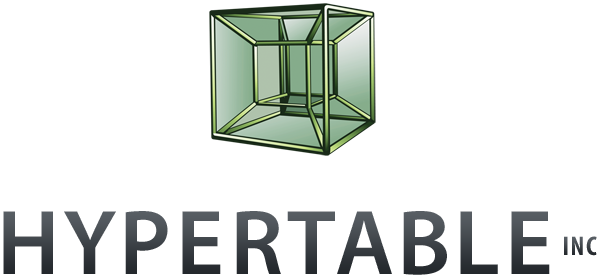
\includegraphics[height=1cm]{img/db/hypertable.png}};
        \end{tikzpicture}
    \end{figure}

    \note{
        Cassandra et HBase sont les exemples les plus connus de systèmes wide-column.
        Bigtable est un modèle fondateur, tandis que Druid vise notamment
        l'analytique et les séries temporelles. Les produits ne sont donc pas
        interchangeables malgré leur classement dans une même famille.
    }
\end{frame}

\begin{frame}{Exemple : distribution des données sur Cassandra}

    \begin{figure}
        \centering
        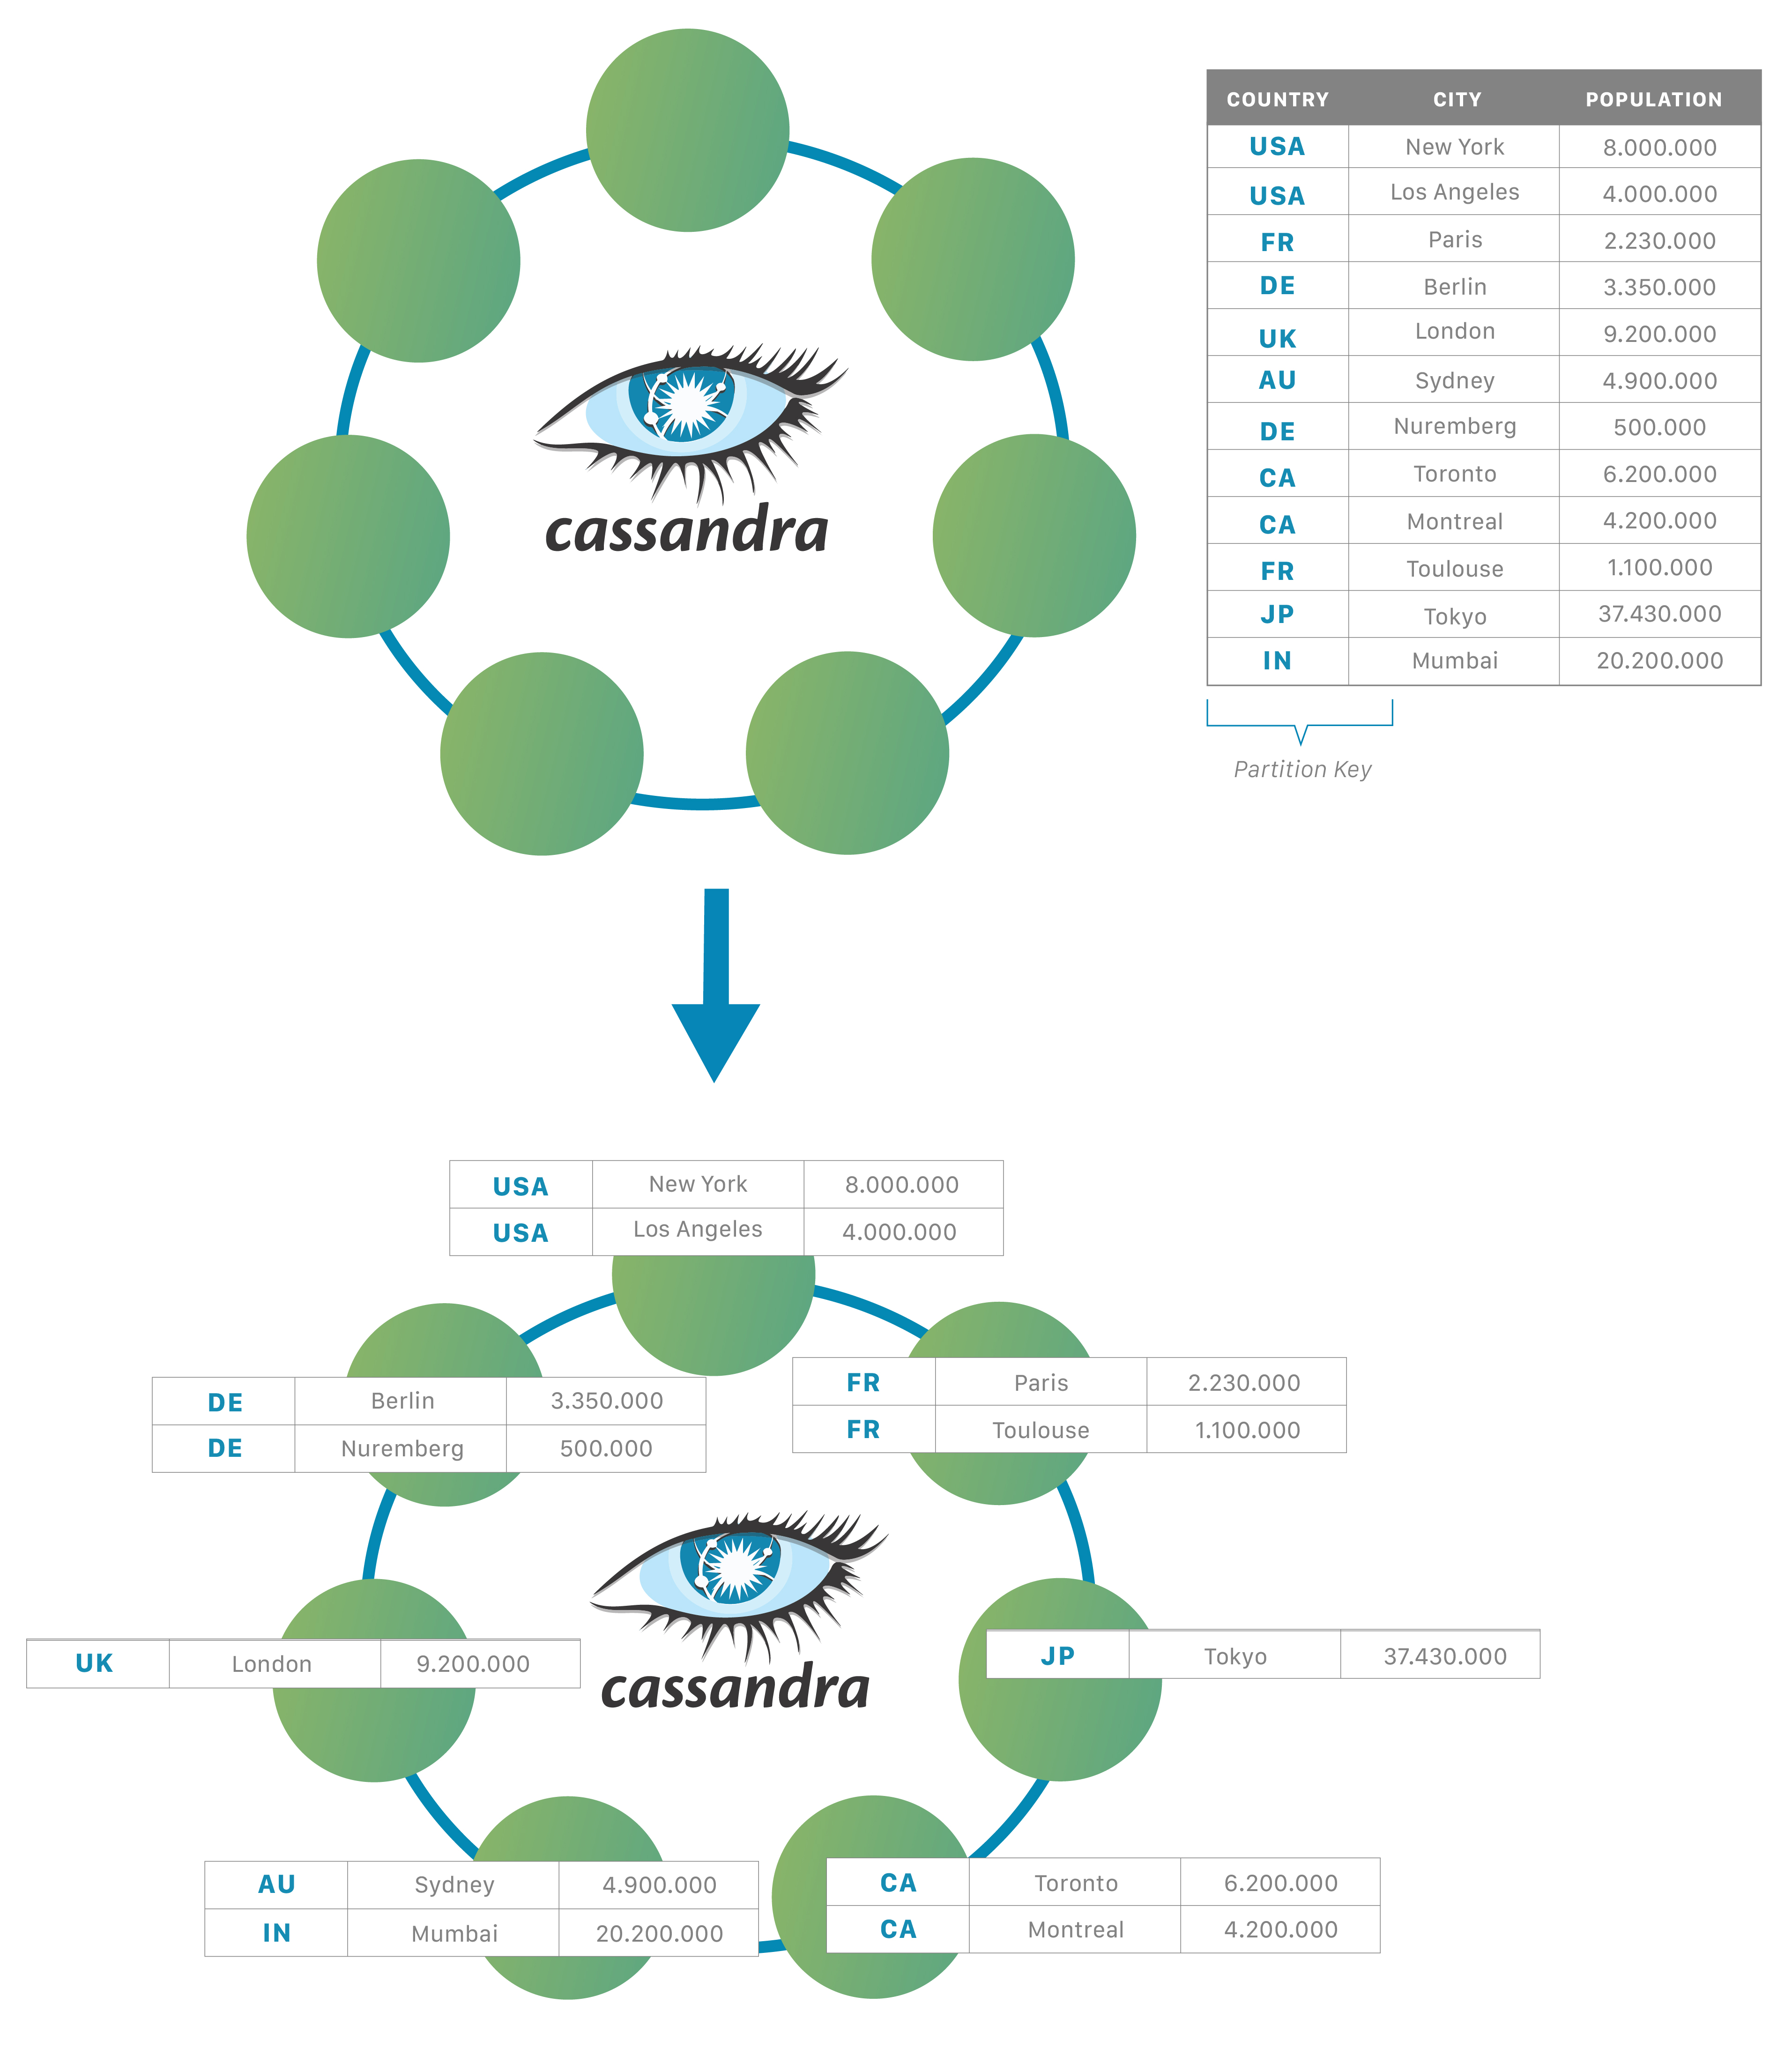
\includegraphics[width=0.8\textheight]{img/apache-cassandra-nodes.jpg}
    \end{figure}

    \note{
        Cassandra distribue les lignes entre les nœuds à partir de la clé
        de partitionnement. Le choix de cette clé est essentiel : elle doit
        répartir la charge tout en permettant les requêtes principales.
        Une mauvaise clé peut créer un nœud très sollicité, appelé hotspot.
    }

\end{frame}

\begin{frame}{Cas d'usages des bases de données orientées colonne}

\begin{itemize}
    \item \textbf{Analytique et data warehousing (OLAP)}\\
    $\hookrightarrow$ Permet d'agréger de grands volumes (SUM, AVG, COUNT sur des millions/milliards de lignes).
    \vspace{0.3cm}

    \item \textbf{Analyse de séries temporelles}\\
    $\hookrightarrow$ Optimisé pour les données IoT, capteurs, logs de monitoring.
    \vspace{0.3cm}

    \item \textbf{Analyses en temps réel}\\
    $\hookrightarrow$ Stocker les informations des utilisateurs et leurs préférences, permettant une extraction rapide pour les recommandations en temps réel.
\end{itemize}

    \note{
        Ces systèmes sont pertinents lorsque le volume, le débit d'écriture
        ou la disponibilité distribuée sont prioritaires. Les analyses financières,
        les événements massifs et les recommandations illustrent des lectures
        ciblées sur des ensembles très volumineux.
        Insister sur le fait que le modèle doit être conçu à partir des requêtes.
    }
\end{frame}

\begin{frame}{Avantages et inconvénients des bases de données colonne}
\vfill
\prosbox{
    \textbf{Avantages}
    \begin{itemize}
        \item Très performant pour les requêtes en lecture sur des colonnes spécifiques.
        \item Scalabilité horizontale adaptée pour le traitement de données massives.
        \item Idéal pour des applications analytiques ou des systèmes OLAP.
    \end{itemize}
}
\vfill
\pause
\consbox{
    \textbf{Inconvénients}
    \begin{itemize}
        \item Moins efficace pour des écritures fréquentes ou des transactions complexes.
        \item Complexité accrue pour gérer les relations entre colonnes.
    \end{itemize}
}
\vfill

    \note{
        Le principal avantage est la combinaison distribution, débit et tolérance
        aux pannes. En revanche, on perd la souplesse d'une base relationnelle
        pour les transactions complexes et les requêtes imprévues.
        Dans Cassandra, on accepte souvent de dupliquer les données dans plusieurs
        tables pour servir efficacement plusieurs requêtes.
    }
\end{frame}
